\documentclass{report}
\usepackage[french]{babel}

% Permet d'ajuster la taille des marges et de la distance pour les footer
\usepackage[tmargin=2cm,rmargin=1in,lmargin=1in,margin=0.85in,bmargin=2cm,footskip=.2in]{geometry}

% Permet d'optimiser l'affichage de différents symboles et formules mathématiques
\usepackage{amsmath,amsfonts,amsthm,amssymb,mathtools}

\usepackage{svg}

% Modifie l'apparence des nombre en mathmode et textmode
\usepackage[varbb]{newpxmath}

% Modifier l'apparence des fractions
\usepackage{xfrac}

% Permet de rayer (barrer) l'argument avec la touche
% \cancel{} \bcancel{} ou \xcancel{}
\usepackage[makeroom]{cancel}

% Extension du package amsmath; corrige certains bugs et déficiences de son prédecesseur
\usepackage{mathtools}

% This package provides most of the flexibility you may want to customize the three basic list
% environments (enumerate, itemize and description)
\usepackage{bookmark} 

% Réorganiser les théorèmes et Lemmes. Usage complexe. 
% Référence : https://ctan.math.illinois.edu/macros/latex/contrib/theoremref/theoremref-doc.pdf
\hypersetup{hidelinks}
\usepackage{hyperref,theoremref} 

% Fournit un environnement pour créer des boîtes colorées
\usepackage[most,many,breakable]{tcolorbox}


%\newcommand\mycommfont[1]{\footnotesize\ttfamily\textcolor{blue}{#1}}\SetCommentSty{mycommfont}

%\newcommand{\incfig}[1]{%\def\svgwidth{\columnwidth}\import{./figures/}{#1.pdf_tex}}
\newcommand{\arc}[1]{\wideparen{#1}}

%Pour colorer les lignes séparatrices de tableaux
\usepackage{colortbl}
\usepackage{tikzsymbols}

\usepackage{framed}
\usepackage{titletoc}
\usepackage{etoolbox}
\usepackage{lmodern}
\usepackage{tabularx}
\usepackage{enumitem}
\usepackage{amsthm}
%==========================================================================================
\usepackage{libris} 
\usepackage{etoolbox}
\usepackage[export]{adjustbox}% for positioning figures

\makeatletter
% Force le chapitre suivant sur la ligne succedant la fin du 
% chapitre précédent
\patchcmd{\chapter}{\if@openright\cleardoublepage\else\clearpage\fi}{}{}{}
\makeatother
\usepackage[Glenn]{fncychap}


%boîte de couleur grise
\tcbset{
  graybox/.style={
    colback=gray!20,
    colframe=black,
    sharp corners=downhill,
    boxrule=1pt,
    left=5pt,
    right=5pt,
    top=5pt,
    bottom=5pt,
    boxsep=0pt,
	 % <-- add four values for each corner
  }
}
\newtcolorbox{graybox}{graybox}

%==========================================================================================



\usepackage{xcolor}
\usepackage{varwidth}
\usepackage{varwidth}
\usepackage{etoolbox}
%\usepackage{authblk}
\usepackage{nameref}
\usepackage{multicol,array}
\usepackage{tikz-cd}
\usepackage[ruled,vlined,linesnumbered]{algorithm2e}
\usepackage{comment} % enables the use of multi-line comments (\ifx \fi) 
\usepackage{import}
\usepackage{xifthen}
\usepackage{pdfpages}
\usepackage{transparent}


%\usepackage[french]{babel}
\usepackage{listings} % pour écrire du code dans un environnement
\lstset{
  basicstyle=\ttfamily,
  columns=fullflexible,
  keepspaces=true
}
\usepackage{caption}
\usepackage{float} % Pour forcer les images au bon endroit



\usepackage[T1]{fontenc}
\usepackage{csquotes}
%%%%%%%%%%%%%%%%%%%%%%%%%%%%%%%%%%%%%%%%%%%%%%%%%%%%%%%%%%%%%%%%%%%%%%%%%%%%%%%%%%%%%%%%%%%%%%%%%
%									ENSEMBLE DE COULEURS
%%%%%%%%%%%%%%%%%%%%%%%%%%%%%%%%%%%%%%%%%%%%%%%%%%%%%%%%%%%%%%%%%%%%%%%%%%%%%%%%%%%%%%%%%%%%%%%%%

\definecolor{myg}{RGB}{56, 140, 70}
\definecolor{myb}{RGB}{45, 111, 177}

\definecolor{mygbg}{RGB}{235, 253, 241}


\definecolor{myr}{RGB}{199, 68, 64}
\definecolor{mytheorembg}{HTML}{F2F2F9}
\definecolor{mytheoremfr}{HTML}{00007B}
\definecolor{mylenmabg}{HTML}{FFFAF8}
\definecolor{mylenmafr}{HTML}{983b0f}
\definecolor{mypropbg}{HTML}{f2fbfc}
\definecolor{mypropfr}{HTML}{191971}
\definecolor{myexamplebg}{HTML}{F2FBF8}
\definecolor{myexamplefr}{HTML}{88D6D1}
\definecolor{myexampleti}{HTML}{2A7F7F}
\definecolor{mydefinitbg}{HTML}{E5E5FF}
\definecolor{mydefinitfr}{HTML}{3F3FA3}
\definecolor{notesgreen}{RGB}{0,162,0}
\definecolor{myp}{RGB}{197, 92, 212}
\definecolor{mygr}{HTML}{2C3338}
\definecolor{myred}{RGB}{127,0,0}
\definecolor{myyellow}{RGB}{169,121,69}
\definecolor{myexercisebg}{HTML}{F2FBF8}
\definecolor{myexercisefg}{HTML}{88D6D1}
\definecolor{myred}{RGB}{127,0,0}
\definecolor{myyellow}{RGB}{169,121,69}

\definecolor{blue}{HTML}{008ED7}
\definecolor{mygray}{gray}{0.75}
\definecolor{lightBlue}{RGB}{235, 245, 255}
\definecolor{tcbcolred}{RGB}{255,0,0}
\definecolor{myGreen}{HTML}{009900}

% command to circle a text
\newtcbox{\entoure}[1][red]{on line,
	arc=3pt,colback=#1!10!white,colframe=#1!50!black,
	before upper={\rule[-3pt]{0pt}{10pt}},boxrule=1pt,
	boxsep=0pt,left=2pt,right=2pt,top=1pt,bottom=.5pt}
% command for the circle for the number of part entries
\newcommand\Circle[1]{\tikz[overlay,remember picture]
	\node[draw,circle, text width=18pt,line width=1pt] {#1};}

\newtcbox{\entouree}[1][red]{on line,
	arc=3pt,colback=#1!10!white,colframe=#1!50!white,
	before upper={\rule[-3pt]{0pt}{10pt}},boxrule=1pt,
	boxsep=0pt,left=2pt,right=2pt,top=1pt,bottom=.5pt}

\newcommand{\shellcmd}[1]{\\\indent\indent\texttt{\footnotesize\# #1}\\}

%=====================================================================
\patchcmd{\tableofcontents}{\contentsname}{\sffamily\contentsname}{}{}
% patching of \@part to typeset the part number inside a framed box in its own line
% and to add color
\makeatletter
\patchcmd{\@part}
  {\addcontentsline{toc}{part}{\thepart\hspace{1em}#1}}
  {\addtocontents{toc}{\protect\addvspace{20pt}}
    \addcontentsline{toc}{part}{\huge{\protect\color{myyellow}%
      \setlength\fboxrule{2pt}\protect\Circle{%
        \hfil\thepart\hfil%
      }%
    }\\[2ex]\color{myred}\sffamily#1}}{}{}

%\patchcmd{\@part}
%  {\addcontentsline{toc}{part}{\thepart\hspace{1em}#1}}
%  {\addtocontents{toc}{\protect\addvspace{20pt}}
%    \addcontentsline{toc}{part}{\huge{\protect\color{myyellow}%
%      \setlength\fboxrule{2pt}\protect\fbox{\protect\parbox[c][1em][c]{1.5em}{%
%        \hfil\thepart\hfil%
%      }}%
%    }\\[2ex]\color{myred}\sffamily#1}}{}{}
\makeatother
% this is the environment used to typeset the chapter entries in the ToC
% it is a modification of the leftbar environment of the framed package
\renewenvironment{leftbar}
  {\def\FrameCommand{\hspace{6em}%
    {\color{myyellow}\vrule width 2pt depth 6pt}\hspace{1em}}%
    \MakeFramed{\parshape 1 0cm \dimexpr\textwidth-6em\relax\FrameRestore}\vskip2pt%
  }
 {\endMakeFramed}

% using titletoc we redefine the ToC entries for parts, chapters, sections, and subsections
\titlecontents{part}
  [0em]{\centering}
  {\contentslabel}
  {}{}
\titlecontents{chapter}
  [0em]{\vspace*{2\baselineskip}}
  {\parbox{4.5em}{%
    \hfill\Huge\sffamily\bfseries\color{myred}\thecontentspage}%
   \vspace*{-2.3\baselineskip}\leftbar\textsc{\small\chaptername~\thecontentslabel}\\\sffamily}
  {}{\endleftbar}
\titlecontents{section}
  [8.4em]
  {\sffamily\contentslabel{3em}}{}{}
  {\hspace{0.5em}\nobreak\itshape\color{myred}\normalfont\contentspage}
\titlecontents{subsection}
  [8.4em]
  {\sffamily\contentslabel{3em}}{}{}  
  {\hspace{0.5em}\nobreak\itshape\color{myred}\contentspage}
%==========================================================================

%PYTHON LSTLISTING STYLE

% Define colors
\definecolor{Pgruvbox-bg}{HTML}{282828}
\definecolor{Pgruvbox-fg}{HTML}{ebdbb2}
\definecolor{Pgruvbox-red}{HTML}{fb4934}
\definecolor{Pgruvbox-green}{HTML}{b8bb26}
\definecolor{Pgruvbox-yellow}{HTML}{fabd2f}
\definecolor{Pgruvbox-blue}{HTML}{83a598}
\definecolor{Pgruvbox-purple}{HTML}{d3869b}
\definecolor{Pgruvbox-aqua}{HTML}{8ec07c}

% Define Python style
\lstdefinestyle{PythonGruvbox}{
	language=Python,
	identifierstyle=\color{lst-fg},
	basicstyle=\ttfamily\color{Pgruvbox-fg},
	keywordstyle=\color{Pgruvbox-yellow},
	keywordstyle=[2]\color{Pgruvbox-blue},
	stringstyle=\color{Pgruvbox-green},
	commentstyle=\color{Pgruvbox-aqua},
	backgroundcolor=\color{Pgruvbox-bg},
	%frame=tb,
	rulecolor=\color{Pgruvbox-fg},
	showstringspaces=false,
	keepspaces=true,
	captionpos=b,
	breaklines=true,
	tabsize=4,
	showspaces=false,
	numbers=left,
	numbersep=5pt,
	numberstyle=\tiny\color{gray},
	showtabs=false,
	columns=fullflexible,
	morekeywords={True,False,None},
	morekeywords=[2]{and,as,assert,break,class,continue,def,del,elif,else,except,exec,finally,for,from,global,if,import,in,is,lambda,nonlocal,not,or,pass,print,raise,return,try,while,with,yield},
	morecomment=[s]{"""}{"""},
	morecomment=[s]{'''}{'''},
	morecomment=[l]{\#},
	morestring=[b]",
	morestring=[b]',
	literate=
	{0}{{\textcolor{Pgruvbox-purple}{0}}}{1}
	{1}{{\textcolor{Pgruvbox-purple}{1}}}{1}
	{2}{{\textcolor{Pgruvbox-purple}{2}}}{1}
	{3}{{\textcolor{Pgruvbox-purple}{3}}}{1}
	{4}{{\textcolor{Pgruvbox-purple}{4}}}{1}
	{5}{{\textcolor{Pgruvbox-purple}{5}}}{1}
	{6}{{\textcolor{Pgruvbox-purple}{6}}}{1}
	{7}{{\textcolor{Pgruvbox-purple}{7}}}{1}
	{8}{{\textcolor{Pgruvbox-purple}{8}}}{1}
	{9}{{\textcolor{Pgruvbox-purple}{9}}}{1}
}
%====================================================================
% 
%====================================================================

% JAVA LSTLISTING STYLE IN Gruvbox Colorscheme
\definecolor{gruvbox-bg}{rgb}{0.282, 0.247, 0.204}
\definecolor{gruvbox-fg1}{rgb}{0.949, 0.898, 0.776}
\definecolor{gruvbox-fg2}{rgb}{0.871, 0.804, 0.671}
\definecolor{gruvbox-red}{rgb}{0.788, 0.255, 0.259}
\definecolor{gruvbox-green}{rgb}{0.518, 0.604, 0.239}
\definecolor{gruvbox-yellow}{rgb}{0.914, 0.808, 0.427}
\definecolor{gruvbox-blue}{rgb}{0.353, 0.510, 0.784}
\definecolor{gruvbox-purple}{rgb}{0.576, 0.412, 0.659}
\definecolor{gruvbox-aqua}{rgb}{0.459, 0.631, 0.737}
\definecolor{gruvbox-gray}{rgb}{0.518, 0.494, 0.471}

\definecolor{lst-bg}{RGB}{45, 45, 45}
\definecolor{lst-fg}{RGB}{220, 220, 204}
\definecolor{lst-keyword}{RGB}{215, 186, 125}
\definecolor{lst-comment}{RGB}{117, 113, 94}
\definecolor{lst-string}{RGB}{163, 190, 140}
\definecolor{lst-number}{RGB}{181, 206, 168}
\definecolor{lst-type}{RGB}{218, 142, 130}


\lstdefinestyle{JavaGruvbox}{
	language=Java,
	basicstyle=\ttfamily\color{lst-fg},
	keywordstyle=\color{lst-keyword},
	keywordstyle=[2]\color{lst-type},
	commentstyle=\itshape\color{lst-comment},
	stringstyle=\color{lst-string},
	numberstyle=\color{lst-number},
	backgroundcolor=\color{lst-bg},
	%frame=tb,
	rulecolor=\color{gruvbox-aqua},
	showstringspaces=false,
	keepspaces=true,
	captionpos=b,
	breaklines=true,
	tabsize=4,
	showspaces=false,
	showtabs=false,
	columns=fullflexible,
	morekeywords={var},
	morekeywords=[2]{boolean, byte, char, double, float, int, long, short, void},
	morecomment=[s]{/}{/},
	morecomment=[l]{//},
	morestring=[b]",
	morestring=[b]',
	numbers=left,
	numbersep=5pt,
	numberstyle=\tiny\color{gray},
}



%====================================================================
% 
%====================================================================


% Define Dracula color scheme for Java
\definecolor{draculawhite-background}{RGB}{237, 239, 252}
\definecolor{draculawhite-comment}{RGB}{98, 114, 164}
\definecolor{draculawhite-keyword}{RGB}{189, 147, 249}
\definecolor{draculawhite-string}{RGB}{152, 195, 121}
\definecolor{draculawhite-number}{RGB}{249, 189, 89}
\definecolor{draculawhite-operator}{RGB}{248, 248, 242}

% Define JavaDraculaWhite lstlisting environment
\lstdefinestyle{JavaDraculaWhite}{
    language=Java,
    backgroundcolor=\color{draculawhite-background},
    commentstyle=\itshape\color{draculawhite-comment},
    keywordstyle=\color{draculawhite-keyword},
    stringstyle=\color{draculawhite-string},
    basicstyle=\ttfamily\small\color{black},
    identifierstyle=\color{black},
    keywordstyle=\color{draculawhite-keyword}\bfseries,
    morecomment=[s][\color{draculawhite-comment}]{/**}{*/},
    showstringspaces=false,
    showspaces=false,
    breaklines=true,
    frame=single,
    rulecolor=\color{draculawhite-operator},
    tabsize=4,  
	numbers=left,
	numbersep=4pt,
	numberstyle=\ttfamily\tiny\color{gray}
}
%====================================================================
% 
%====================================================================
% Define PythonDraculaWhite lstlisting environment 
\definecolor{draculawhite-bg}{HTML}{FAFAFA}
\definecolor{draculawhite-fg}{HTML}{282A36}
\definecolor{pdraculawhite-keyword}{HTML}{BD93F9}

\definecolor{pdraculawhite-comment}{HTML}{6272A4}
\definecolor{draculawhite-number}{HTML}{FF79C6}


\lstdefinestyle{PythonDraculaWhite}{
    language=Python,
    basicstyle=\ttfamily\small\color{draculawhite-fg},
    backgroundcolor=\color{draculawhite-background},
    keywordstyle=\color{orange}\bfseries,
    stringstyle=\color{draculawhite-string},
    commentstyle=\color{pdraculawhite-comment}\itshape,
    numberstyle=\color{draculawhite-number},
    showstringspaces=false,
	showspaces=false,
    breaklines=true,
	frame=single,
	rulecolor=\color{draculawhite-operator}, 
    tabsize=4,
    morekeywords={as,with,1,2,3,4, 5,6,7,8,9,True,False},
    %escapeinside={(*@}{@*)},
    numbers=left,
    numbersep=5pt,
    %xleftmargin=15pt,
    %framexleftmargin=15pt,
    %framexrightmargin=0pt,
    %framexbottommargin=0pt,
    %framextopmargin=0pt,
    %rulecolor=\color{draculawhite-fg},
    %frame=tb,
    %aboveskip=0pt,
    %belowskip=0pt,
    %captionpos=b,
	numberstyle=\ttfamily\tiny\color{gray} 
}
%====================================================================
% 
%====================================================================

% Define colors for HTML langage
\definecolor{html-orange}{HTML}{FF5733}
\definecolor{html-yellow}{HTML}{F0E130}
\definecolor{html-green}{HTML}{50FA7B}
\definecolor{html-blue}{HTML}{5AFBFF}
\definecolor{html-purple}{HTML}{BD93F9}
\definecolor{html-pink}{HTML}{FF80BF}
\definecolor{html-gray}{HTML}{6272A4}
\definecolor{html-white}{HTML}{F8F8F2}

% Defines a new HTML5 langage that extend on the html langange
\lstdefinestyle{HTMLDraculaWhite}{
  language=HTML,
  backgroundcolor=\color{html-white},
  basicstyle=\ttfamily\color{html-gray},
  keywordstyle=\color{html-blue},
  stringstyle=\color{html-orange},
  commentstyle=\color{html-green},
  tagstyle=\color{html-yellow},
  moredelim=[s][\color{html-pink}]{<!--}{-->},
  moredelim=[s][\color{html-purple}]{\{}{\}},
  showstringspaces=false,
  tabsize=2,
  breaklines=true,
  columns=fullflexible,
  %frame=single,
  framexleftmargin=5mm,
  xleftmargin=10mm,
  numbers=left,
  numberstyle=\tiny\color{html-gray},
  escapeinside={<@}{@>}
}

%====================================================================
% 
%====================================================================
% Define the colors needed for the HTMLDraculaDark environment
\definecolor{htmltag}{HTML}{ff79c6}
\definecolor{htmlattr}{HTML}{f1fa8c}
\definecolor{htmlvalue}{HTML}{bd93f9}
\definecolor{htmlcomment}{HTML}{6272a4}
\definecolor{htmltext}{HTML}{f8f8f2}
\definecolor{htmlbackground}{HTML}{282a36}

% Define the HTMLDraculaDark environment
\lstdefinestyle{HTMLDraculaDark}{
    basicstyle=\ttfamily\color{htmltext},
    commentstyle=\color{htmlcomment},
    keywordstyle=\color{htmltag},
    stringstyle=\color{htmlvalue},
    emph={DOCTYPE,html,head,body,div,span,a,script},
    emphstyle={\color{htmltag}\bfseries},
    sensitive=true,
    showstringspaces=false,
    backgroundcolor=\color{htmlbackground},
    %frame=tb,
    language=HTML,
    tabsize=4,
    breaklines=true,
    breakatwhitespace=true,
    numbers=left,
    numbersep=5pt,
    numberstyle=\tiny\color{htmlcomment},
    escapeinside={<@}{@>},
	rulecolor=\color{htmlbackground}
}
%====================================================================
% 
%====================================================================






% Crée un environnement "Theorem" numéroté en fonction du document
\tcbuselibrary{theorems,skins,hooks} 
\newtcbtheorem{Theorem}{Théorème}
{%
	enhanced,
	breakable,
	colback = mytheorembg,
	frame hidden,
	boxrule = 0sp,
	borderline west = {2pt}{0pt}{mytheoremfr},
	sharp corners,
	detach title,
	before upper = \tcbtitle\par\smallskip,
	coltitle = mytheoremfr,
	fonttitle = \bfseries\fontfamily{lmss}\selectfont,
	description font = \mdseries\fontfamily{lmss}\selectfont,
	separator sign none,
	segmentation style={solid, mytheoremfr},
}
{thm}

% Crée un environnement "Preuve" numéroté en fonction du document
\tcbuselibrary{theorems,skins,hooks}
\newtcbtheorem{Preuve}{Preuve.}
{
	enhanced,
	breakable,
	colback=white,
	frame hidden,
	boxrule = 0sp,
	borderline west = {2pt}{0pt}{mytheoremfr},
	sharp corners,
	detach title,
	before upper = \tcbtitle\par\smallskip,
	coltitle = mytheoremfr,
	description font=\fontfamily{lmss}\selectfont,
	fonttitle=\fontfamily{lmss}\selectfont\bfseries,
	separator sign none,
	segmentation style={solid, mytheoremfr},
}
{th}


% Crée un environnement "Preuve" numéroté en fonction du document
\tcbuselibrary{theorems,skins,hooks}
\newtcbtheorem{Explication}{Explication}
{
	enhanced,
	breakable,
	colback=white,
	frame hidden,
	boxrule = 0sp,
	borderline west = {2pt}{0pt}{mytheoremfr},
	sharp corners,
	detach title,
	before upper = \tcbtitle\par\smallskip,
	coltitle = mytheoremfr,
	description font=\fontfamily{lmss}\selectfont,
	fonttitle=\fontfamily{lmss}\selectfont\bfseries,
	separator sign none,
	segmentation style={solid, mytheoremfr},
}
{th}




% Crée un environnement "Example" numéroté en fonction du document
\tcbuselibrary{theorems,skins,hooks}
\newtcbtheorem{Example}{Exemple.}
{
	enhanced,
	breakable,
	colback=lightBlue,
	frame hidden,
	boxrule = 0sp,
	borderline west = {2pt}{0pt}{myb},
	sharp corners,
	detach title,
	before upper = \tcbtitle\par\smallskip,
	coltitle = myb,
	description font=\fontfamily{lmss}\selectfont,
	fonttitle=\fontfamily{lmss}\selectfont\bfseries,
	separator sign none,
	segmentation style={solid, mytheoremfr},
}
{th}



% Crée un environnement "EExample" numéroté en fonction du document
\tcbuselibrary{theorems,skins,hooks}
\newtcbtheorem{EExample}{Exemple.}
{
	enhanced,
	breakable,
	colback=white,
	frame hidden,
	boxrule = 0sp,
	borderline west = {2pt}{0pt}{myb},
	sharp corners,
	detach title,
	before upper = \tcbtitle\par\smallskip,
	coltitle = myb,
	description font=\mdseries\fontfamily{lmss}\selectfont,
	fonttitle=\fontfamily{lmss}\selectfont\bfseries,
	separator sign none,
	segmentation style={solid, mytheoremfr},
}
{th}



% Crée un environnement "Lemme" numéroté en fonction du document
\tcbuselibrary{theorems,skins,hooks}
\newtcbtheorem{Lemme}{Lemme}
{
	enhanced,
	breakable,
	colback=mylenmabg,
	frame hidden,
	boxrule = 0sp,
	borderline west = {2pt}{0pt}{mylenmafr},
	sharp corners,
	detach title,
	before upper = \tcbtitle\par\smallskip,
	coltitle = mylenmafr,
	description font=\mdseries\fontfamily{lmss}\selectfont,
	fonttitle=\fontfamily{lmss}\selectfont\bfseries,
	separator sign none,
	segmentation style={solid, mytheoremfr},
}
{th}


\tcbuselibrary{theorems,skins,hooks}
\newtcbtheorem{PreuveL}{Preuve.}
{
	enhanced,
	breakable,
	colback=white,
	frame hidden,
	boxrule = 0sp,
	borderline west = {2pt}{0pt}{mylenmafr},
	sharp corners,
	detach title,
	before upper = \tcbtitle\par\smallskip,
	coltitle = mylenmafr,
	description font=\fontfamily{lmss}\selectfont,
	fonttitle=\fontfamily{lmss}\selectfont\bfseries,
	separator sign none,
	segmentation style={solid, mytheoremfr},
}
{th}


\newtcbtheorem{Remarque}{Remarque.}
{
	enhanced,
	breakable,
	colback=white,
	frame hidden,
	boxrule = 0sp,
	borderline west = {2pt}{0pt}{myb},
	sharp corners,
	detach title,
	before upper = \tcbtitle\par\smallskip,
	coltitle = myb,
	description font=\mdseries\fontfamily{lmss}\selectfont,
	fonttitle=\fontfamily{lmss}\selectfont\bfseries,
	separator sign none,
	segmentation style={solid, mytheoremfr},
}
{th}


\newtcbtheorem{DefG}{Définition}
{
	enhanced,
	breakable,
	colback=mygbg,
	frame hidden,
	boxrule = 0sp,
	borderline west = {2pt}{0pt}{myg},
	sharp corners,
	detach title,
	before upper = \tcbtitle\par\smallskip,
	coltitle = myg,
	description font=\mdseries\fontfamily{lmss}\selectfont,
	fonttitle=\fontfamily{lmss}\selectfont\bfseries,
	separator sign none,
	segmentation style={solid, mytheoremfr},
}
{th}



% Crée une boîte ayant la même couleur que l'environnement theorem.
\tcbuselibrary{theorems,skins,hooks}
\newtcolorbox{Theoremcon}
{%
	enhanced
	,breakable
	,colback = mytheorembg
	,frame hidden
	,boxrule = 0sp
	,borderline west = {2pt}{0pt}{mytheoremfr}
	,sharp corners
	,description font = \mdseries
	,separator sign none
}

% Crée un environnement "Definition" numéroté en fonction de la section
\newtcbtheorem[number within=chapter]{Definition}{Définition}{enhanced,
	before skip=2mm,after skip=2mm, colback=red!5,colframe=red!80!black,boxrule=0.5mm,
	attach boxed title to top left={xshift=1cm,yshift*=1mm-\tcboxedtitleheight}, varwidth boxed title*=-3cm,
	boxed title style={frame code={
			\path[fill=tcbcolback!10!red]
			([yshift=-1mm,xshift=-1mm]frame.north west)
			arc[start angle=0,end angle=180,radius=1mm]
			([yshift=-1mm,xshift=1mm]frame.north east)
			arc[start angle=180,end angle=0,radius=1mm];
			\path[left color=tcbcolback!10!myred,right color=tcbcolback!10!myred,
			middle color=tcbcolback!60!myred]
			([xshift=-2mm]frame.north west) -- ([xshift=2mm]frame.north east)
			[rounded corners=1mm]-- ([xshift=1mm,yshift=-1mm]frame.north east)
			-- (frame.south east) -- (frame.south west)
			-- ([xshift=-1mm,yshift=-1mm]frame.north west)
			[sharp corners]-- cycle;
		},interior engine=empty,
	},
	fonttitle=\bfseries,
	title={#2},#1}{def}

% Crée un environnement "definition" numéroté en fonction du Chapitre
\newtcbtheorem[number within=section]{definition}{Définition}{enhanced,
	before skip=2mm,after skip=2mm, colback=red!5,colframe=red!80!black,boxrule=0.5mm,
	attach boxed title to top left={xshift=1cm,yshift*=1mm-\tcboxedtitleheight}, varwidth boxed title*=-3cm,
	boxed title style={frame code={
			\path[fill=tcbcolback]
			([yshift=-1mm,xshift=-1mm]frame.north west)
			arc[start angle=0,end angle=180,radius=1mm]
			([yshift=-1mm,xshift=1mm]frame.north east)
			arc[start angle=180,end angle=0,radius=1mm];
			\path[left color=tcbcolback!60!black,right color=tcbcolback!60!black,
			middle color=tcbcolback!80!black]
			([xshift=-2mm]frame.north west) -- ([xshift=2mm]frame.north east)
			[rounded corners=1mm]-- ([xshift=1mm,yshift=-1mm]frame.north east)
			-- (frame.south east) -- (frame.south west)
			-- ([xshift=-1mm,yshift=-1mm]frame.north west)
			[sharp corners]-- cycle;
		},interior engine=empty,
	},
	fonttitle=\bfseries,
	title={#2},#1}{def}

\usetikzlibrary{arrows,calc,shadows.blur}
\tcbuselibrary{skins}
\newtcolorbox{note}[1][]{%
	enhanced jigsaw,
	colback=gray!20!white,%
	colframe=gray!80!black,
	size=small,
	boxrule=1pt,
	title=\textbf{Note : },
	halign title=flush center,
	coltitle=black,
	breakable,
	drop shadow=black!50!white,
	attach boxed title to top left={xshift=1cm,yshift=-\tcboxedtitleheight/2,yshifttext=-\tcboxedtitleheight/2},
	minipage boxed title=1.5cm,
	boxed title style={%
		colback=white,
		size=fbox,
		boxrule=1pt,
		boxsep=2pt,
		underlay={%
			\coordinate (dotA) at ($(interior.west) + (-0.5pt,0)$);
			\coordinate (dotB) at ($(interior.east) + (0.5pt,0)$);
			\begin{scope}
				\clip (interior.north west) rectangle ([xshift=3ex]interior.east);
				\filldraw [white, blur shadow={shadow opacity=60, shadow yshift=-.75ex}, rounded corners=2pt] (interior.north west) rectangle (interior.south east);
			\end{scope}
			\begin{scope}[gray!80!black]
				\fill (dotA) circle (2pt);
				\fill (dotB) circle (2pt);
			\end{scope}
		},
	},
	#1,
}


% Crée un environnement "qstion" 
\newtcbtheorem{qstion}{Question}{enhanced,
	breakable,
	colback=white,
	colframe=mygr,
	attach boxed title to top left={yshift*=-\tcboxedtitleheight},
	fonttitle=\bfseries,
	title={#2},
	boxed title size=title,
	boxed title style={%
		sharp corners,
		rounded corners=northwest,
		colback=tcbcolframe,
		boxrule=0pt,
	},
}{def}


% Pour créer un environnement "Liste" 

\tcbuselibrary{theorems,skins,hooks}
\newtcbtheorem[number within=section]{Liste}{Liste}
{%
	enhanced
	,breakable
	,colback = myp!10
	,frame hidden
	,boxrule = 0sp
	,borderline west = {2pt}{0pt}{myp!85!black}
	,sharp corners
	,detach title
	,before upper = \tcbtitle\par\smallskip
	,coltitle = myp!85!black
	,fonttitle = \bfseries\sffamily
	,description font = \mdseries
	,separator sign none
	,segmentation style={solid, myp!85!black}
}
{th}


\tcbuselibrary{theorems,skins,hooks}
\newtcbtheorem{Syntaxe}{Syntaxe.}
{%
	enhanced
	,breakable
	,colback = myp!10
	,frame hidden
	,boxrule = 0sp
	,borderline west = {2pt}{0pt}{myp!85!black}
	,sharp corners
	,detach title
	,before upper = \tcbtitle\par\smallskip
	,coltitle = myp!85!black
	,fonttitle = \bfseries\fontfamily{lmss}\selectfont 
	,description font = \mdseries\fontfamily{lmss}\selectfont 
	,separator sign none
	,segmentation style={solid, myp!85!black}
}
{th}



% Crée un environnement "Concept" numéroté en fonction du document
\tcbuselibrary{theorems,skins,hooks}
\newtcbtheorem{Concept}{Concept.}
{
	enhanced,
	breakable,
	colback=mylenmabg,
	frame hidden,
	boxrule = 0sp,
	borderline west = {2pt}{0pt}{mylenmafr},
	sharp corners,
	detach title,
	before upper = \tcbtitle\par\smallskip,
	coltitle = mylenmafr,
	description font=\mdseries\fontfamily{lmss}\selectfont,
	fonttitle=\fontfamily{lmss}\selectfont\bfseries,
	separator sign none,
	segmentation style={solid, mytheoremfr},
}
{th}


% Crée un environnement "codeEx" numéroté en fonction du document
\tcbuselibrary{theorems,skins,hooks}
\newtcbtheorem{codeEx}{Exemple.}
{
	enhanced,
	breakable,
	colback=white,
	frame hidden,
	boxrule = 0sp,
	borderline west = {2pt}{0pt}{gruvbox-bg},
	sharp corners,
	detach title,
	before upper = \tcbtitle\par\smallskip,
	coltitle = gruvbox-bg,
	description font=\mdseries\fontfamily{lmss}\selectfont,
	fonttitle=\fontfamily{lmss}\selectfont\bfseries,
	separator sign none,
	segmentation style={solid, mytheoremfr},
}
{th}


% Crée un environnement "codeEx" numéroté en fonction du document
\tcbuselibrary{theorems,skins,hooks}
\newtcbtheorem{codeRem}{Remarque.}
{
	enhanced,
	breakable,
	colback=white,
	frame hidden,
	boxrule = 0sp,
	borderline west = {2pt}{0pt}{gruvbox-bg},
	sharp corners,
	detach title,
	before upper = \tcbtitle\par\smallskip,
	coltitle = gruvbox-bg,
	description font=\mdseries\fontfamily{lmss}\selectfont,
	fonttitle=\fontfamily{lmss}\selectfont\bfseries,
	separator sign none,
	segmentation style={solid, mytheoremfr},
}
{th}










\title{\Huge{IFT1025 Programmation 2}\\De Python à Java}
\author{\huge{Franz Girardin}}
\date{3 Mai 2023}
\lstset{inputencoding=utf8/latin1}
%====================================================================

%====================================================================
\begin{document}

\maketitle

\newpage
\pdfbookmark[section]{\contentsname}{toc}
\tableofcontents
\pagebreak
%====================================================================
% 
%====================================================================
\chapter{Introduction}


\section{Particularité de Java et Python}
\begin{Concept*}{Langage statique et langage dynamique}{}
	\textbf{Java} est un langage statique; la vérification du code est effectuée \textit{lors de la compilation}. 
	\textbf{Python} est un langage dynamique et la vérification est donc en cours 
	\textit{tout au long de l'exécution de programme}. 
\end{Concept*}

\begin{DefG*}{Vérification de code}{}
	Il s'agit du processus de vérification et d'application des contraintes de types en fonction de la syntaxe
	permise par le langage. 

\end{DefG*}



\begin{table}[h]
		\caption {Comparaison de Python et Java}

	\begin{center}
		\begin{tabular}{m{7cm}|m{7cm}}

	\arrayrulecolor{blue}\hline
	\rowcolor{lightBlue}
	\textcolor{myb}{\bfseries\fontfamily{lmss}\selectfont{Python}} & 
	\textcolor{myb}{\bfseries\fontfamily{lmss}\selectfont{Java}}
	\\
	\hline
	\arrayrulecolor{black}
	\footnotesize\textit{\texttt{Langage interprété}}	
	& 
	\footnotesize\textit{\texttt{Lanagage compilé}}
	\\
	\hline	
	\footnotesize\textit{\texttt{Typage dynamique}} et faible quantité de type & 
	\footnotesize\textit{\texttt{Typage statique}} grande variété de types
	\\
	\hline
	\footnotesize\textit{\texttt{Langage tolérant et peu rigide}} & 
	\footnotesize\textit{\texttt{Langage rigide qui permet peu d'erreurs}}
	\\
	\hline
	\footnotesize\textit{\texttt{Développement plus simple mais exécution plus lente}} & 
	\footnotesize\textit{\texttt{Développement plus complexe et exécution plus rapide}}
	\\
	\hline
	\end{tabular}
	\end{center}
\end{table}


\begin{EExample*}{Hello world! en Python}{}
\begin{lstlisting}[style=PythonDraculaWhite]	
print("Hello world!")
\end{lstlisting}
\end{EExample*}

\begin{EExample*}{Hello world! en Java}{}
\begin{lstlisting}[style=JavaDraculaWhite]
	public class Example {
		public static void main(String[] args) {
			System.out.println("Hello world!");
		}
	}
\end{lstlisting}\end{EExample*}


\begin{Concept*}{Compilation de Java}
	Le code Java est d'abord transformé en bytecode—un langage intermédiaire.

\end{Concept*}
 
\noindent Java est un langage de programmation orienté objet. Le code qu'on écrit est donc parti d'une classe; la classe principale—
\entoure[gray]{\texttt{\footnotesize{main}}} dans ce cas-ci. La classe main a une méthode : \entouree[gray]{\texttt{\footnotesize{public static void main (String[] args) \{...\}}}}. Le programme qu'on écrit est généralement compris entre les crochets de
la méthode \entouree[gray]{\texttt{\footnotesize{main}}}
%====================================================================
% 
%====================================================================
\chapter{Notions Essentielles}
\section{Types Java}
\begin{DefG*}{Types}{}
	Un type définit la nature des valeur que peut prendre une donnée et les opérateurs qui peuvent lui être 
	appliqués. 
\end{DefG*}
 

\begin{note}
Les programmes qui explicitent les types optimisent le traitement et la vitesse d'exécution du code,
utilisent moins d'espace mémoire et tendent à engendrer moins d'erreur.
\end{note}


\begin{table}[h]
		\caption{ Types primitifs Java}

	\begin{center}
		\begin{tabular}{l|l}

	\arrayrulecolor{blue}\hline
	\rowcolor{lightBlue}
	\textcolor{myb}{\fontfamily{lmss}\selectfont{\textbf{Type}}} & 
	\textcolor{myb}{\fontfamily{lmss}\selectfont{\textbf{Description}}}
	\\
	\hline
	\arrayrulecolor{black}
	\footnotesize\texttt{short} & \footnotesize\textit{\texttt{Entier encodé sur 16 bits}}  
	\\
	\hline	
	\texttt{\footnotesize{int}} & \footnotesize\textit{\texttt{Entier encodé sur 32 bits}}
	\\
	\hline
	\texttt{\footnotesize{long}} & \footnotesize\textit{\texttt{Entier encodé sur 64 bits}}
	\\
	\hline
	\texttt{\footnotesize{float}} & \footnotesize\textit{\texttt{Nombre à virgule encodé sur 32 bits}}
	\\
	\hline
	\texttt{\footnotesize{double}} & \footnotesize\textit{\texttt{Nombre à virgule encodé sur 64 bits}}
	\\
	\hline
	\texttt{\footnotesize{boolean}} & \footnotesize\textit{\texttt{Valeur de vérité}} 
	\entouree[gray]{\texttt{\footnotesize{true}}} \footnotesize\textit{\texttt{ou}} 
	\entouree[gray]{\texttt{\footnotesize{false}}}
	\\
	\hline
	\texttt{\footnotesize{char}} & \footnotesize\textit{\texttt{Caractère textuel unitque}}
	\\
	\hline
	\texttt{\footnotesize{byte}} & \footnotesize\textit{\texttt{Nombre entier de 8 bits}}
	\\
	\hline 
	\end{tabular}
	\end{center}
\end{table}


\begin{codeRem*}{}{}
Le type d'une variable est précisé lors de la déclaration. Après la déclaration, le type est immuable. 
\end{codeRem*}



\begin{EExample*}{Déclaration de variable en Java}{}
\begin{lstlisting}[style=JavaDraculaWhite]
// On declare un variable en precisant son type
int a = 0;

// Formule invalide puisque a precedemment definit ne peut contenir que des entiers
a = "Bonjour !";

String b = "abc";

// Formule invalide puisque b precedemment definit ne peut etre un booleen
b = true; 
\end{lstlisting}
\end{EExample*}


\begin{EExample*}{Déclaration de variable en Python}{}
\begin{lstlisting}[style=PythonDraculaWhite]
# Toutes ces operations sont permises 
a = "Hello World!"
a = 5
a = True
b = False 
\end{lstlisting}	
\end{EExample*}

\begin{Remarque*}{Entiers et décimaux}{}
Par défaut, les nombnres entiers littéraux sont des int et les nombrs décimaux littéraux sont des doubles 
\end{Remarque*}
\begin{EExample*}{}{}
\begin{lstlisting}[style=JavaDraculaWhite]
int age = 25;
double nombreDecimal = 123456789.0;

// On utilise le suffixe L pour specifier un "long int"
long grandNombreEntier = 12345678910L

// On utilise le suffixe f pour specifier un float de 32 bits
float nombreFlottant32bits = 15.3f;

boolean isCoffeeCold = false;

// On utilise le guillemet simple pour specifier un char (caractere textuel unique)
char caractere = 'a'; 

\end{lstlisting}
\end{EExample*}

\begin{note}
	Le \textit{résultat des opérations} dépend du types des variables; le résultat peut être arrondis selon le \textbf{type des opérandes} 
\end{note}


\begin{EExample*}{Arithmétique selon le type}{}
\begin{lstlisting}[style=JavaDraculaWhite]
	// Addition et division de deux double
	double a = 3.0;
	double b = 2.0;

	System.out.println(a+b); //Affiche 5.0 (un double). 

	System.out.print(a/b); // Affiche 1.5 (un double)
\end{lstlisting}

\begin{lstlisting}[style=JavaDraculaWhite]
	// Addition et division de deux int
	int a = 3;
	int b = 2;

	System.out.println(a + b) // Affiche 5 (un int)

	System.out.pintln(a/b); // Affiche 1 (un int)
\end{lstlisting}
\end{EExample*}




\begin{Syntaxe*}{Changer le type grâce à un cast}{}
	On peut \textit{forcer le changement d'un type} pour effectuer une opération arithétique en utilisant un \textit{cast}. On précise entre parenthèse le type désiré suivit de la variable à modifier. 
\end{Syntaxe*}

\begin{EExample*}{}{}
\begin{lstlisting}[style=JavaDraculaWhite]
int a = 3;
int b = 2;

/Affiche 1.5
System.out.println(double) a / (double) b);
\end{lstlisting}
\end{EExample*}



\begin{note}
Les entiers sont automatiquement convertit vers leur équivalent le plus large si nécessaiere 
\\
\texttt{\footnotesize{byte -> short -> int -> long -> float -> double }}
\end{note}

\begin{EExample*}{Conversion automatique d'un int}{}
\begin{lstlisting}[style=JavaDraculaWhite]
	int a = 3;
	
	//, L'entier sera convertit en double pour effectuer l'operation 
	System.out.println(a / 2.0); //Affiche 1.5
\end{lstlisting}
\end{EExample*}

\begin{Syntaxe*}{Forcer un perte de précision grâce à un cast}{}
	On peut forcer un \textit{type plus précis} à devenir moins précis lors d'un opération toujours en utilisant un cast


\end{Syntaxe*}	
\begin{EExample*}{}{}
\begin{lstlisting}[style=JavaDraculaWhite]
	double c = 3.0
	double d = 2.0

	/* Afficherait normalement 1.5, car c est un double 
	et le calcul se ferait sur double */
	System.out.println(c / 2);

	/* Affiche 1 car les deux opérandes de 
	la division sont des entiers */
	System.out.println( (int) c / (int) d); 
\end{lstlisting}
\end{EExample*}

\begin{note}
Un cast de \entouree[gray]{\texttt{\footnotesize{float}}} en \entouree[gray]{\texttt{\footnotesize{int}}} a comme effet de tronquer la partie fractionnaire, plutôt que d'arrondir le résultat. 
\end{note}

\begin{EExample*}{}{}
	\begin{lstlisting}[style=JavaDraculaWhite]
		System.out.println((int) 4.6); // Affichera 4
		System.out.println((int) -4.6); 
		// Affichera -4 (aurait affiche -5 si cast arrondissait) 
	\end{lstlisting}
\end{EExample*}

%====================================================================
% 
%====================================================================
\section{Fonctions Java}
\begin{Concept*}{Fonction principale}
	La \textit{première fonction d'un programme Java} est \entoure[gray]{\texttt{\footnotesize{public static void main(String args[])}}}. Elle contient géralement tout le reste du code. 
\end{Concept*}

\noindent Lorsqu'on déclare une fonction, on doit spécifier le \textit{type des arguments} qu'elle prends et le
\textit{type de la valeur retournée} par la fonction.

\begin{EExample*}{Fonction de base}{}
	\begin{lstlisting}[style=JavaDraculaWhite]
		
		// La declaration int avant carre indique que la fonction retourne des entiers
		public static int carre(int x) {
		    return x * x
		/* La declaration int entre parenthese et avant le x indique que 
		la fonction accepte des entiers */
		}
	\end{lstlisting}
\end{EExample*}

\begin{DefG*}{Signature d'une fonction}{}
	Il s'agit de la combinaison de son nom et du type de ses arguments. La fonction de l'example précédent a
	comme signature \entoure[gray]{\texttt{\footnotesize{carre(int)}}}.
\end{DefG*}

\begin{Concept*}{Portée d'une variable}
	Il s'agit de la partie du programme où la variable est accessible. Une variable locale est un variable définit
	dans une fonction donnée et accessible uniquement à cette fonction 
	\textit{ou les éléments faisant parti du bloc de cette fonction}.

\end{Concept*}
	\begin{DefG*}{Bloc}{}
	Il s'agit d'une portion de code qui est délémitée par des accolades 
	\entouree[gray]{\texttt{\footnotesize{\{...\}}}} 

\end{DefG*}


\noindent Lorsqu'une fonction ne retourne aucune valeur, on l'indique en écrivant 
\entouree[gray]{\texttt{\footnotesize{void}}} avant le nom de la fonction. Les fonctions qui ne retournent rien
sont ne sont pas des fonctions mais plutôt des \textit{procédures}. 

\begin{EExample*}{Fonction sans valeur de retour}{}
\begin{lstlisting}[style=JavaDraculaWhite]
	public static void direBonjour () {
	System.out.println("Bonjour !");
	}
\end{lstlisting}
\end{EExample*}
%====================================================================
% 
%====================================================================
\section{Tableaux Java}
\begin{Syntaxe*}{Création d'un tableau en Java}{}
	On ne peut avoir qu'un type par tableau en Java. Lorsqu'on déclare le tableau, il faut 
	\textit{spécifier le type des éléments qu'il contient}. Il faut aussi spécifier la quantité 
	d'éléments et \textit{manuellement initialiser le tableau}.
\end{Syntaxe*}

\begin{EExample*}{Initialisation manuelle et automatique d'un tableau Java}{}
	\begin{lstlisting}[style=JavaDraculaWhite]
		
        // La commande new int permet de creer un tableau vide de taille N
		int[] a = new int[3];

		// On specifie les valeurs a chaque position du tableau 
		a[0] = 1;
		a[1] = 2;
		a[3] = 3;
        
		/* On peut aussi initialiser automatiquement avec un tableau litteral
		Java comprend qu'on veut un tableau de taille 5 */
		int[] b = {1,2,3,4,5,6}
	\end{lstlisting}
\end{EExample*}
\begin{Remarque*}{Trouver la taille d'un tableau}{}
On peut déterminer la quantité d'éléments présents dans un 
tableau en utilisant la commande \entouree[gray]{\texttt{\footnotesize{NomDuTableau.length}}}
\end{Remarque*}
\begin{EExample*}{}{}
\begin{lstlisting}[style=JavaDraculaWhite]
	// Génère un tableau d'entiers contenant trois éléments 
	int [] tab = {10, 20, 30};

    // Affiche 3 (la taille du tableau)
	System.out.println(tab.length); 

\end{lstlisting}
\end{EExample*}


\begin{Syntaxe*}{Tableau 2D}{}
Il s'agit d'un tableau dans lequel chaque élément est également un tableau à une dimension.  
\end{Syntaxe*}
\begin{EExample*}{Création d'un tableau 2D}{}
\begin{lstlisting}[style=JavaDraculaWhite]
/* Methode manuelle : on cree un tableau a deux dimensions 
"[2]" ou chaque element est un tableau de taille 3.*/ 
   int[][] a = new int[2][5]

/* Methode automatique : Java comprend qu'on veut creer un 
tableau de taille 2 dans lequel chaque element est un tableau de taile 3 */
int [][] b = {{1,2,3,} {4,5,6}}
\end{lstlisting}
\end{EExample*}



\begin{note}
On ne peut pas comparer la taile de deux tableau via
l'opérateur \entouree[gray]{\texttt{\footnotesize{==}}} ; Java
considère qu'on veut comparer deux zones mémoires.
\end{note}
\begin{Syntaxe*}{Comparaison de tableau}{}
\entouree[gray]{\texttt{\footnotesize{Arrays.equals(tableau1, tableau2}}} vérifie si \texttt{\footnotesize{tableau1}} a la même taille que \texttt{\footnotesize{tableau2}}.

\entouree[gray]{\texttt{\footnotesize{Arrays.deepEquals(tableau1, tableau2}}} vérifie récursivement \textit{si les tableaux multidimensionnels} on la même taille.
\end{Syntaxe*}


\begin{note}
On ne peut pas ajouter des éléments à un tableau Java; chaque tableau est de taille fixe. 
\end{note}

\begin{Syntaxe*}{Ajouter un élément à un tableau}{}
Dans l'ordre, il faut créer un tableau de taille N + 1; copier
les N premiers éléments du tableau original; et ajouter un élément de plus.
\end{Syntaxe*}


\begin{EExample*}{Ajout d'élément par création d'un nouveau tableau}{}
\begin{lstlisting}[style=JavaDraculaWhite]
	public static void main(String[] args) {
	int[] t {10,20,30}; // Cree un tableau de 3 elements

	// Cree un nouveau tableau de 4 elements 
	int[] temp = new int[t.length + 1];

	//Copie les element existants de t dans temp
	for(int i=0; i<t.length; i++)
		temp[i] = t[i];

	// Ajoute l'element desire a la fin du tableau 
	temp[t.length] = 40;
	
	// Assigne la valeur du tableau temp au tableau t
	t = temp
\end{lstlisting}
\end{EExample*}

\begin{note}
Lorsqu'on souhaite retier un élément d'un tableau, le même 
principe s'applique : Crée un tableau de taille N - 1; 
copier les N - 1 éléments à conserver dans le nouveau tableau;assigner la valeur du nouveau tableau à l'ancient tableau.
\end{note}

\section{Chaîne de caractères \textit{string}}
\begin{Concept*}{Stockage des string}
	L'enregistrement d'un string en mémoire implique la conversion dudit caractère en chiffre selon un standard—p. ex. ASCII.
\end{Concept*}

\begin{EExample*}{Création d'un string Java}{}
\begin{lstlisting}[style=JavaDraculaWhite]
	String nom = "Jimmy Whooper";
	char[] tDeChar = {'1','I', 'F', 'G', '5'};
\end{lstlisting}
\end{EExample*}

\begin{note}
L'opérateur \entouree[gray]{\texttt{\footnotesize{+}}} sert 
autant à l'addition de nombres qu'à la concaténation de Strings
\end{note}

\begin{EExample*}{Concaténation de Strings}{}
\begin{lstlisting}[style=JavaDraculaWhite]
	String phrase = "Bonjour mon ami.";

	// Affiche : "Bonjour mon ami. Comment vas-tu ?"
    System.out.println(phrase + " Comment vas-tu ?");

	// Affiche "1020" ; la concatenation des deux Strings.
	System.out.println("10" + "20");
\end{lstlisting}
\end{EExample*}

\begin{note}
Lorsqu'on une des opérandes est de type 
\texttt{\footnotesize{String}}, l'autre est converti en 
\texttt{\footnotesize{String}} et l'opération effectuée
est une concaténation. La valeur résultante est \textit{de type String}.	 
\end{note}

\begin{EExample*}{Concaténation de String à un int}{}
\begin{lstlisting}[style=JavaDraculaWhite]
	System.out.println(25 + "10"); //Affiche "2510"
	
	int b = 123;
	System.out.println("a" + b); // Affiche "a123"
\end{lstlisting}
\end{EExample*}

\begin{note}
On utilise la méthode 
\entouree[gray]{\texttt{\footnotesize{.length}}} 
pour retourner le nombre d'éléments d'une chaîne de
caractères. Un espace vaut \textit{1 caractère}. Le nombre
retourné est de type int. 
\end{note}

\begin{EExample*}{Déterminer la taille du chaîne}{}
	\begin{lstlisting}[style=JavaDraculaWhite]
		"Allo".length() // vaut 4

		String phrase = "Bonjour mon ami";
		phrase.length() // vaut 16

		(" 25"+10.;length() // vaut 5 (l'espace est compté)
	\end{lstlisting}
\end{EExample*}

\begin{note}
Un String est une chaîne de caractères 
\entoure[gray]{\texttt{\footnotesize{char}}}.
Chaque \entouree[gray]{\texttt{\footnotesize{char}}} d'un
String a un index \textit{en fonction de sa position dans le String}.
\end{note}


\begin{EExample*}{}{}
	\begin{lstlisting}[style=JavaDraculaWhite]
		char B = "Nom";
		// B a le char 'N' en position 0
		// B a le char 'o' en position 1
		// B a le char 'm' en position 2
	\end{lstlisting}
\end{EExample*}

\begin{note}
On peut obtenir le caractère d'un String \texttt{\footnotesize{s}} à la position \texttt{\footnotesize{i}} grâce à la
commande \entouree[gray]{\texttt{\footnotesize{s.charAt(i)}}}
\end{note}

\begin{EExample*}{Obtenir le caractère à une position donnée d'un String}{}
	\begin{lstlisting}[style=JavaDraculaWhite]
		"Allo".charAt(0) /* vaut 'A' de type char
		ne vaut pas "A" qui serait de type String */

		String n = "123"
		n.charAt(n.length()-1) // vaut '3' (et non pas "3")
		n.charAt(3) // engendre une erreur ; n'a pas de position 3
		(n + 0).charAt(3) // vaut '0' (et non "0", ni 0)
	\end{lstlisting}
\end{EExample*}

\begin{note}
On peut extraire une partie d'un String grâce à la méthode 
\entouree[gray]{\texttt{\footnotesize{s.substring(debut, fin)}}}. Le resultat de cette expression est une sous-chaîne de
\texttt{\footnotesize{s}}.
\end{note}

\begin{Remarque*}{}{}
La nouvelle chaîne crée par la commande
\entouree[gray]{\texttt{\footnotesize{s.substring(debut, fin)}}} comment à la position \texttt{\footnotesize{debut}} et se
termine avant la position \texttt{\footnotesize{fin}}.
La longeur de la sous-chaîne est donc \texttt{\footnotesize{fin - debut}}
\end{Remarque*}

\begin{EExample*}{Création de sous-chaîne}{}
\begin{lstlisting}[style=JavaDraculaWhite]
	//Vaut "onjour"
	"Bonjour".substring(1,6)

	String salut = "Allo";
	int pos = 0;

    //Vaut ""
	salut.substring(pos, pos) 
	salut.sustring(pos, pos+1) // vaut "A" (et non pas 'A')
	salut.substring(pos, pos+2) //vaut "Al"

	salut.substring(0, salut.length()-1) // vaut "All"
	salut.substrong(salut.length()-1, salut.length()) // vaut "o"
\end{lstlisting}
\end{EExample*}


\begin{EExample*}{Modifier le \entouree[gray]{\texttt{\footnotesize{char}}} d'un String à la position i}{}
	\begin{lstlisting}[style=JavaDraculaWhite]
		// Soit i == 1
		int i = 1;

		String salut2 =  salut.substring(0,i) + 'X' +
		    salut.substring(i+1, salut.length());
		// salut2 vaut "AXlo"
	\end{lstlisting}
\end{EExample*}

\begin{note}
La méthode \entouree[gray]{\texttt{\footnotesize{.toUpperCase()}}} retourne une version où toutes les miniscules ont été 
transformées en majuscules. On utilise plutôt \entouree[gray]{\texttt{\footnotesize{.toLowerCase()}}} pour obtenir une
version où toutes les majuscules sont changées en minuscules. 

\end{note}

\begin{EExample*}{Changement de majuscules et minuscules}{}
\begin{lstlisting}[style=JavaDraculaWhite]
	"BonJour!".toUpperCase() // vaut "BONJOUR!"
    "BonJour!".toLowerCase() // vaut "bonjour!"
\end{lstlisting}
\end{EExample*}

\begin{note}
On ne peut pas comparer deux String via l'opérateur ==; Java
considère qu'on veut comparer deux zones mémoires. 
\end{note}

\begin{Syntaxe*}{Comparaison de deux String}{}
\entouree[gray]{\texttt{\footnotesize{StringA.equals(StringB)}}} permet de comparer la longueur des String \texttt{\footnotesize{A}} et \texttt{\footnotesize{B}}. La case est sensible.
On utilisera \entouree[gray]{\texttt{\footnotesize{.equalsIgnoreCase()}}} si on ne veut pas que la case soit sensible lors
de la comparaison. 
\end{Syntaxe*}


\begin{EExample*}{Comparer deux String en Java}{}
	\begin{lstlisting}[style=JavaDraculaWhite]
		String a = "gazoline"
        String b = "gazoline"

        System.out.println(a == b) // Affiche false
		System.out.println(a.quals(b)); //Affiche true
	
		System.out.println(("gaz" + "oline").equals("gazoline"))
		// Affiche true

		System.out.println("abc".equals("ABC"));
		// Affiche false ; la case est importante
		System.out.println("aBc".equals("abc"));
		// Affiche false


		System.out.println("abc".equalsIgnoreCase("ABC"));
		// Affiche true
		System.out.println("aBc".equalsIgnoreCase("abc"));
		// Affiche true
	\end{lstlisting}
\end{EExample*}

\begin{DefG*}{Ordre lexicographique}{}
Il s'agit de l'ordre dans lequel on place un String par 
rapport à un autre, en fonction de sa valeur—sachant que chaque char qui compose le string a une valeur déterminée par l'ordre alphabétique. 
\end{DefG*}

\begin{note}
On peut utiliser la méthode \entouree[gray]{\texttt{\footnotesize{compareTo()}}} pour déterminer quel String précède l'autre.
\end{note}

\begin{EExample*}{Comparaison de l'ordre lexicographique}{}
\begin{lstlisting}[style=JavaDraculaWhite]
	"ABC".compreTo("ABC")
	// Vaut 0 puisque les deux String sont identiques 

	"ABC".compareTo("ABZ") 
	// A une valeur negative puisque C precede Z.

	"ABZ".compareTo("ABC")
	// Vaut un entier positif, pusique Z > C

	"ABC.compareTo("ABCDEFGH")
	// Vaut un entier positif puisque "ABZ" est considere
	comme plus grand que "ABCDEFGH"
\end{lstlisting}
\end{EExample*}

\begin{note}
La comparaison lexicographique se fait avec la valeur 
numérique du code Unicode du caractère coresspondant. L'ordre
de priorité est le suivant : 
\texttt{\footnotesize{chifres < lettres majuscules < lettres minuscules}}
\end{note}

\begin{figure}[H]
\centering

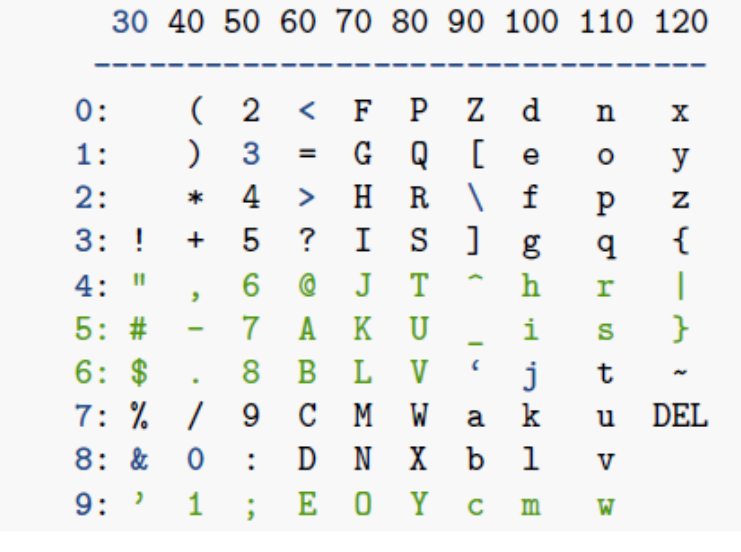
\includegraphics[width=0.45\linewidth]{StringLexico}
\end{figure}

\begin{note}
On peut ignorer la lors de la comparaison grâce à la commande
\entouree[gray]{\texttt{\footnotesize{compareToIgnoreCase()}}}
\end{note}

\begin{EExample*}{Comparaison en Ignorant la case}{}
\begin{lstlisting}[style=JavaDraculaWhite]
	"ABc".compareToIgnoreCase("ABZ") 
	// Vaut 0 puirsque "abc" == "abc"
\end{lstlisting}
\end{EExample*}

\begin{Syntaxe*}{Déterminer l'index d'une sous-chaîne}{}
On peut utiliser la comande \entouree[gray]{\texttt{\footnotesize{.indexOf()}}} pour identifier la position à laquelle on trouve une sous-chaîne X. Si la chapine ne contient pas la
sous-chaîne recherchée, la commande \textbf{retourne -1}.
\end{Syntaxe*}

\begin{EExample*}{}{}
\begin{lstlisting}[style=JavaDraculaWhite]
	/* Soit une chaine ; pour trouver la positon de X = jour
	dans la chaîne on utilise : */
	"Bonjour Monsieur!".indexOf("jour") 
	// Vaut 3 (int); jour débute  à la position 3 du String.
	"Bonjour Monsieur!".indexOf("jours")
	// Vaut -1 ; la sous-chaine n'existe pas
\end{lstlisting}
\end{EExample*}

\begin{note}
On peut spécifier la position à partir de laquelle il faut chercher l'index en fournissant \textit{second paramètre} à la commande \entouree[gray]{\texttt{\footnotesize{String.indexOf()}}}
\end{note}

\begin{EExample*}{Trouver l'index en spécifiant le début de la sous-chaîne}{}
	\begin{lstlisting}[style=JavaDraculaWhite]
		"Bonjour Monsieur!".indexOf("on",0)
		//Vaut 1
		"Bonjour Monsieur!".indexOf("on", 5) 
		// Vaut 9 ; le premier "on" trouve a partir de la position 5
		"Bonjour Monsieur!".indexOf("on", 10) 
		// Vaut -1 ; "on" est introuvable apres la position 10.
	\end{lstlisting}
\end{EExample*}

\begin{note}
On peut également utiliser un \texttt{\footnotesize{char}} 
à la place d'un \texttt{\footnotesize{String}} pour
effectuer la recherche. Exemple \entouree[gray]{\texttt{\footnotesize{"Bonjour".indexOf('j') $\leftrightarrow$ \\
"Bonjour".indexOf("j")}}}
\end{note}

\begin{Syntaxe*}{Convertir un type primitif en entier}{}
On \textbf{ne peut pas} utiliser de cast. Il faut utiliser la formule \entouree[gray]{\texttt{\footnotesize{valeur + ""}}}. 
Alternativement, on peut utiliser la commande 
\entouree[gray]{\texttt{\footnotesize{String.valueOf()}}} 
\end{Syntaxe*}

\begin{EExample*}{Convertir un type primitif en entier}{}
\begin{lstlisting}[style=JavaDraculaWhite]
	10 + "" // Vaut "10"
	128.7 + "" // Vaut "128.7" et est de type String

	String.valueOf(10) // Vaut "10"
	boolean a = true;
	a + "" // Vaut "true"
	String.valueOf(a) // Vaut "true"
\end{lstlisting}
\end{EExample*}

\begin{Syntaxe*}{Convertir un String représentant un nombre en un entier}{}
Les commandes \entouree[gray]{\texttt{\footnotesize{TypeVoulu.parseTypevoulu}}} permet la conversion \texttt{\footnotesize{String de nombre}} $rightarrow$ \texttt{\footnotesize{int}}.
\end{Syntaxe*}

\begin{EExample*}{Conversion String de nombre $\rightarrow$ int}{}
\begin{lstlisting}[style=JavaDraculaWhite]
	Integer.parseInt("1" + "2") // Vaut 12 et est de type int
	Double.parseDouble("-3e-1" // Vaut -0.3 et est de type Double.
	Integer.parseInt("bonjour") // Engendre un erreur a l'execution
\end{lstlisting}
\end{EExample*}
%====================================================================
% 
%====================================================================
\section{Entrées et Sorties}
\begin{Syntaxe*}{Affichage à l'écran}{}
On utilise \entouree[gray]{\texttt{\footnotesize{System.out.println}}} pour effectuer un saut à la ligne lors de l'affiche. La commande \entouree[gray]{\texttt{\footnotesize{System.out.print}}} affiche \textit{sans saut à la ligne}. 
\end{Syntaxe*}
\begin{Syntaxe*}{Interaction avec l'utilisateur}{}
La commande \entouree[gray]{\texttt{\footnotesize{args}}} permet d'enregistrer et manipuler des arguments 
\textit{de la ligne de commande}. La commande \entouree[gray]{\texttt{\footnotesize{Scanner}}} permet la lecture
de données interactives. 
\end{Syntaxe*}

\begin{EExample*}{Utilisation d'arguments en ligne de commande}{}
\begin{lstlisting}[style=JavaDraculaWhite]
	public class Hello {
	    public static void main(String[] args) {
		// Le code va ici
		System.out.println("Hello, " + arg[0] + " !");
		}
	}
\end{lstlisting}
\end{EExample*}
\begin{note}
la variable args est un tableau de Strings. Chaque argument présenté au lancement du programme est un
\textit{String qui est enregistré dans la variable args}. 
\end{note}

\begin{EExample*}{}{}
\begin{lstlisting}[style=JavaDraculaWhite]
	public class Max {

	    public static void main(String[] args) {
			int max = -1
			
			for (int i=0, i<args.length; i++) {
				max = Math.max(max, Integer.parseInt(args[i]));
			}

			System.out.println("Maxumum=" + max);
		}
	}
	/* Execution :
	$ javac Max.java
	$ java Max 1 6 3 1 5 3
	Maximum=6
	*/
\end{lstlisting}
\end{EExample*}
%====================================================================
% 
%====================================================================
\
section{Modèle Mémoire}
\begin{Concept*}{Mémoire d'un programme}
Elle est conceptuellement séparée en deux partie : \textit{la pile} et \textit{le tas}.
\end{Concept*}
\pagebreak
\begin{center}
\begin{figure}[H]
	\includegraphics[width=1\linewidth]{Lecture01MindMap.pdf}
\end{figure}
\end{center}

















\end{document}
